\chapter*{Anhang}
% =================================================================
\thispagestyle{fancy} \addcontentsline{toc}{chapter}{Anhang}
% =================================================================
\section*{Messresultate \glqq Bestimmen der Eigenfrequenz\grqq}
\begin{figure}[h]
\centering
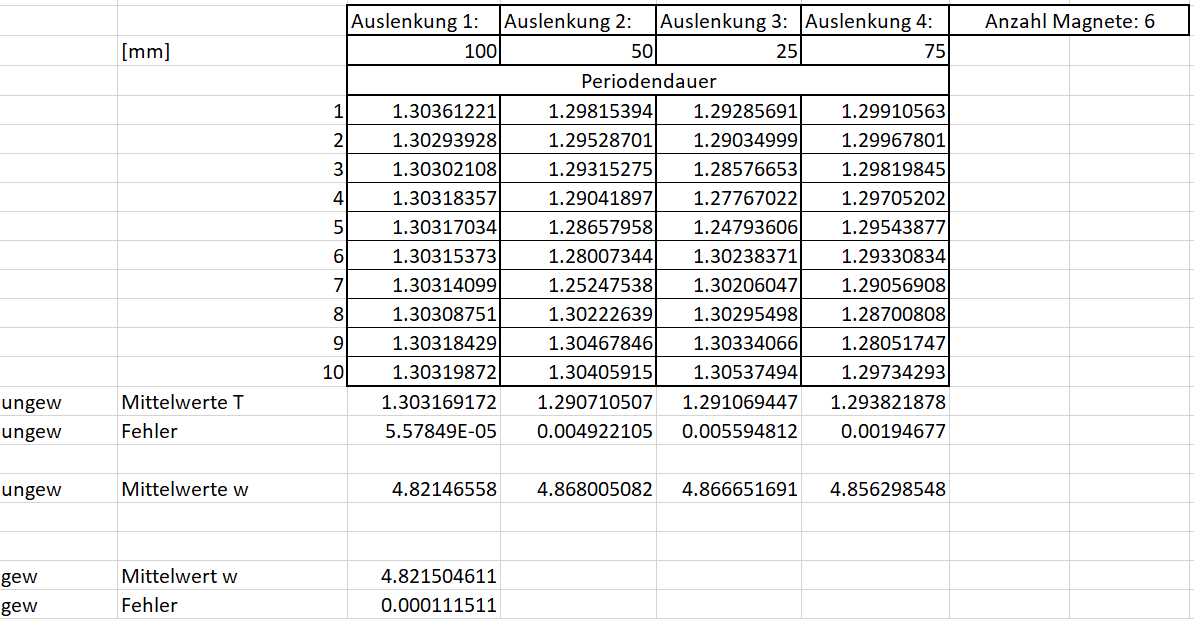
\includegraphics[scale=0.8]{Bilder/messungen_eigenfrequenz.png} 
\caption{Messresultate mit den gewichteten und ungewichteten Mittelwerten und Fehlern}
\label{fig:messresultate_bestimmen_eigenfrequenz}
\end{figure}
\section*{Messresultate \glqq Amplitudenverlauf\grqq}
\begin{figure}[h]
\centering
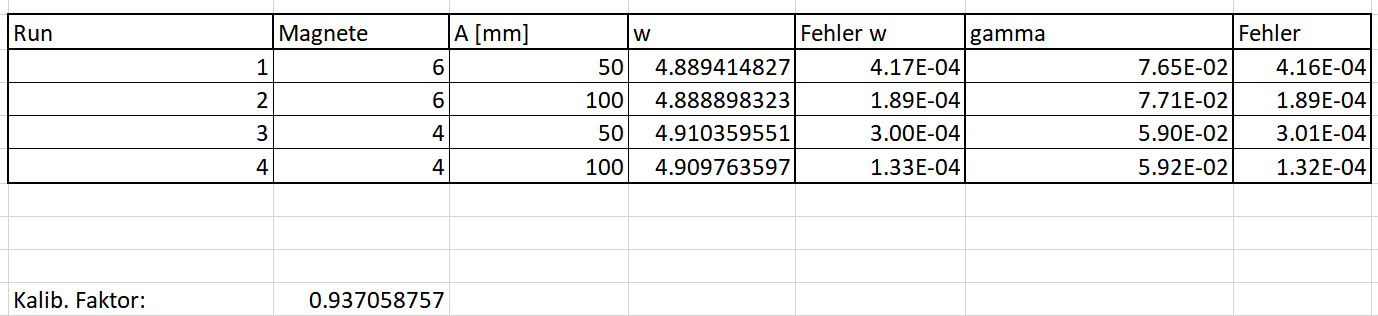
\includegraphics[scale=0.73]{Bilder/messungen_amplitudenverlauf.png} 
\caption{Amplitudenverlauf mit dem Kalibrierungsfaktor um die Zeitdaten anzupassen wegen des schlechten Clocks des Laser Distanzmessgeräts}
\label{fig:messresultate_amplitudenverlauf}
\end{figure}
\newpage
\section*{Messresultate \glqq Amplituden- und Phasenresonanz\grqq}
\begin{figure}[h]
\centering
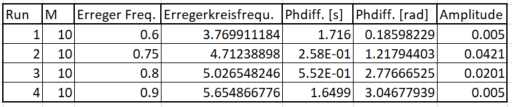
\includegraphics[scale=1.3]{Bilder/messungen_phasenresonanz.png} 
\caption{Messresultate für die Bestimmung der Amplituden- und Phasenresonanz}
\label{fig:messresultate_phasenresonanz}
\end{figure}
\section*{Amplitudenverläufe}
\begin{figure}[h]
\centering
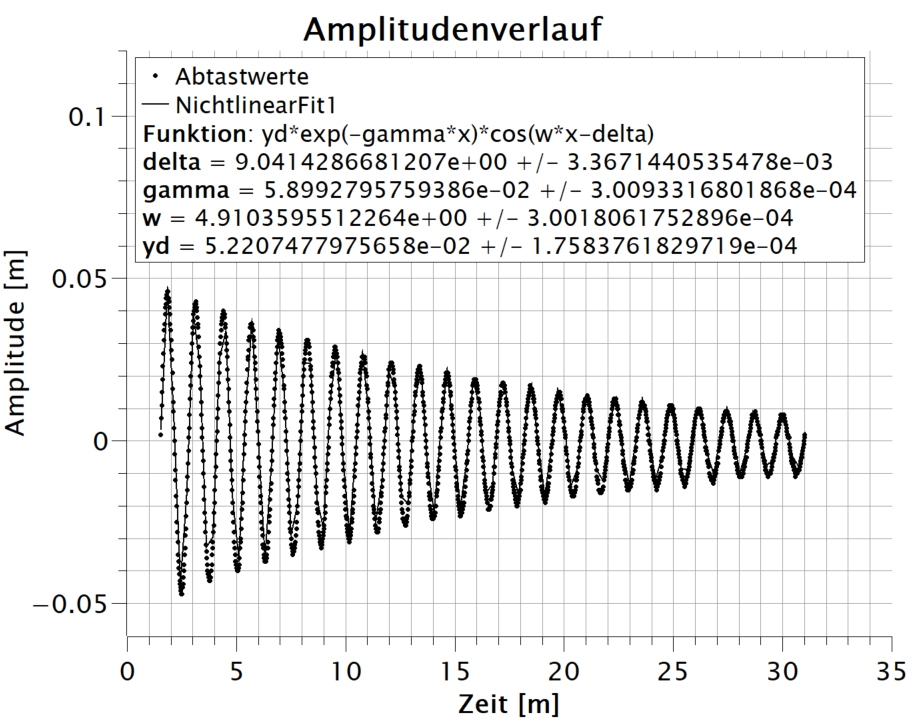
\includegraphics[scale=1]{Bilder/amplitudenverlauf_005_4.png} 
\caption{Amplitudenverlauf; Startauslenkung: $0.05m$, Anzahl Magnete: 4}
\label{fig:amplitudenverlauf_005_4}
\end{figure}
\newpage
\begin{figure}[h]
\centering
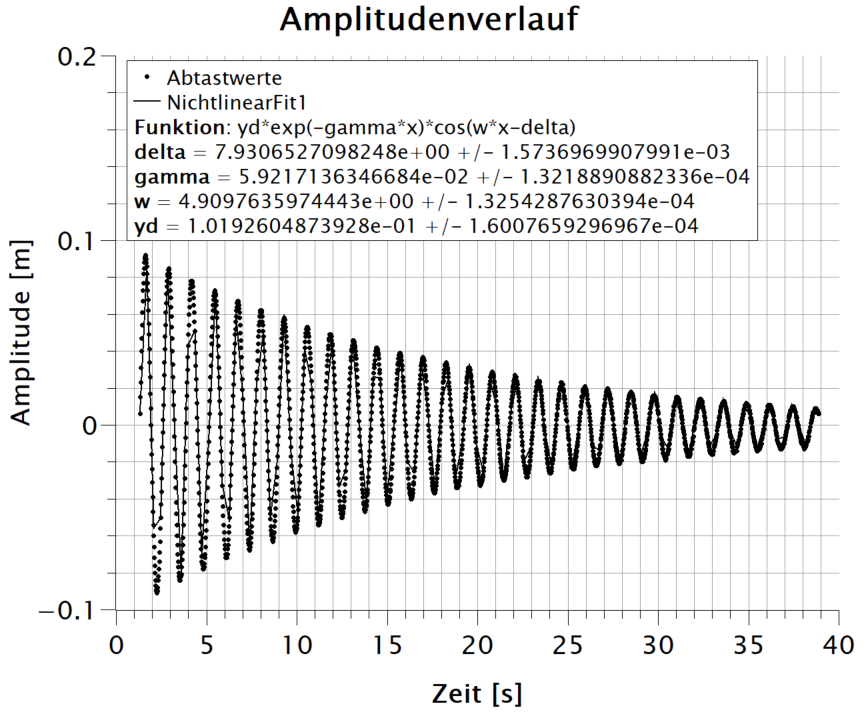
\includegraphics[scale=1.1]{Bilder/amplitudenverlauf_01_4.png} 
\caption{Amplitudenverlauf; Startauslenkung: $0.1m$, Anzahl Magnete: 4}
\label{fig:amplitudenverlauf_01_4}
\end{figure}
\newpage
\begin{figure}[h]
\centering
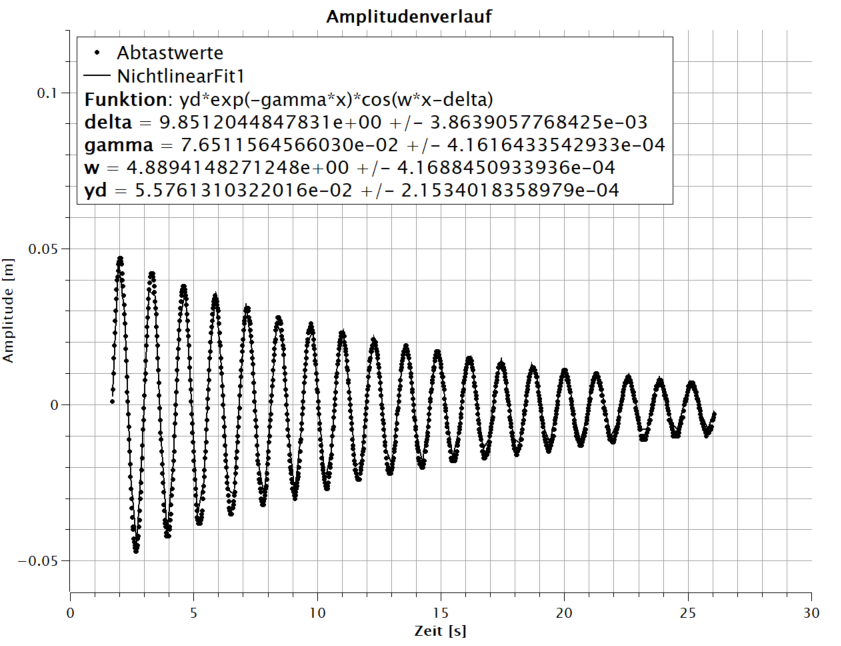
\includegraphics[scale=1.2]{Bilder/amplitudenverlauf_005_6.png} 
\caption{Amplitudenverlauf; Startauslenkung: $0.05m$, Anzahl Magnete: 6}
\label{fig:amplitudenverlauf_005_6}
\end{figure}
\newpage